%\section{Experiments}
%\label{sec:experiments}

\section{Experiments}
We use Fetch push, reach and pick and place
tasks~\citep{plappert201802multigoalrl} in our experiments:
%
\begin{description}
  \item[Fetch-Reach] The tip of a robotic arm reaching a desired location.
  \item[Fetch-Push] A robotic arm pushing a block to a desired location.
  \item[Fetch-Slide] A robotic arm sliding a puck to a desired location.
\end{description}%
% 
\subsection{Baseline: Hindsight experience replay}
Hindsight Experience Replay~\cite{andrychowicz2016learning} targets
goal-conditioned tasks.
In goal-conditioned tasks, the rewards can be very sparse. Unless the agent hits
the goal, no value-able reward is learned and rest of the space is almost even
with respect to the rewards. To address this challenge, HER first assumes that
for every $\state_t$ the achieved goal $\goal_t = f_\goal(\state_t)$ is known.
Then HER simulates as if the achieved goal $\goal_t$ was the intended goal all
along by re-sampling the goal conditioned reward function.
More concretely, two time steps $t_1$ and $t_2 > t_1$ from the same episode in the replay memory are
sampled. The achieved goal at $t_2$ , $\goal_{t_2}$ is assumed to be the desired
goal at $t_1$ and the new simulated transition becomes $(\state_{t_1},
\act_{t_1}, \state_{t_1 + 1}, \Rew(\state_{t_1}, \goal_{t_2}, \act_{t_1}))$,
where $\Rew(\state_{t_1}, \goal_{t_2}, \act_{t_1})$ is the recomputed reward
instead of the observed reward $\Rew(\state_{t_1}, \goal^*_{e}, \act_{t_1})$ that
depends on the desired goal $\goal^*_{e}$ for that episode $e$.

HER can be applied to either DDPG or DQN, the experiments in
\citet{andrychowicz2016learning} show them to be applied on DDPG.



%
\begin{figure}
  \def\frac{0.32}
  On Fetch Push\\
  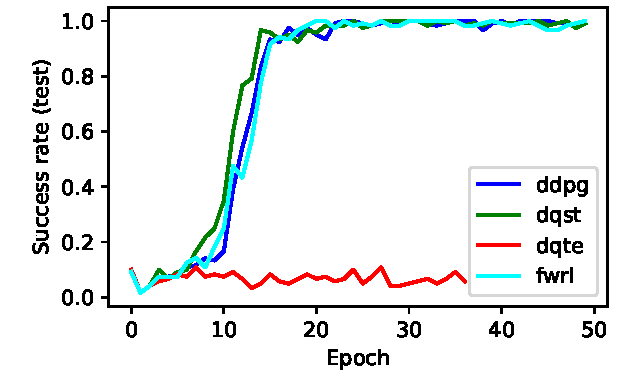
\includegraphics[width=\frac\columnwidth]{media/res/38f4625-FetchPush-v1-fwrl-future/test/success_rate.pdf}%
  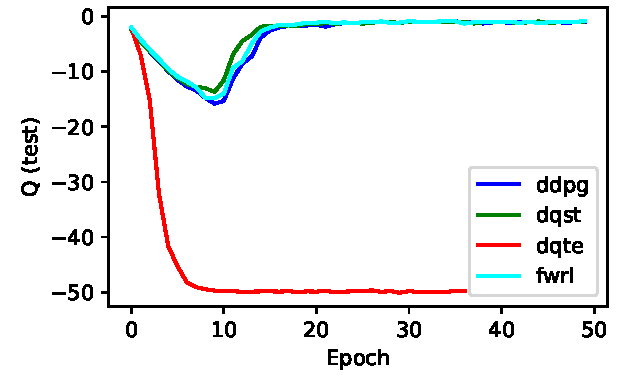
\includegraphics[width=\frac\columnwidth]{media/res/38f4625-FetchPush-v1-fwrl-future/test/mean_Q.pdf}%
  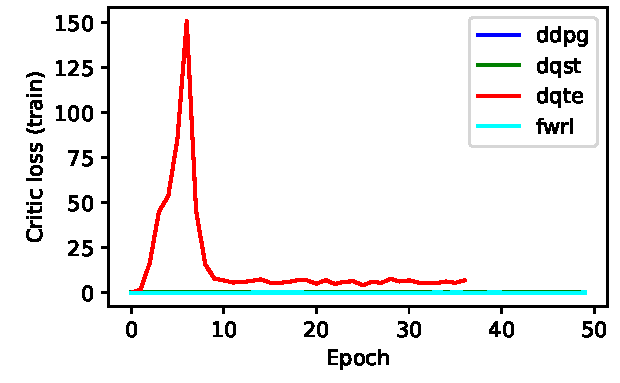
\includegraphics[width=\frac\columnwidth]{media/res/38f4625-FetchPush-v1-fwrl-future/train/critic_loss.pdf}\\
  On Fetch Reach\\
  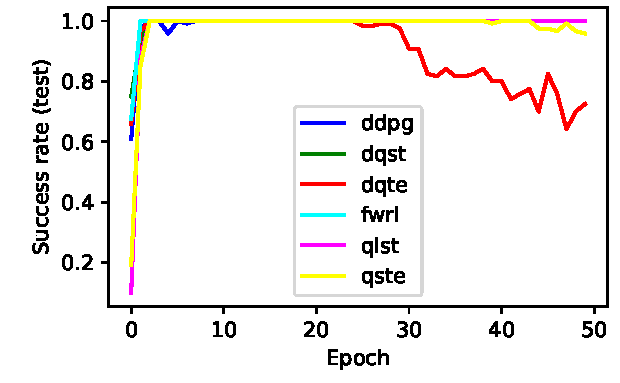
\includegraphics[width=\frac\columnwidth]{media/res/38f4625-FetchReach-v1-fwrl-future/test/success_rate.pdf}%
  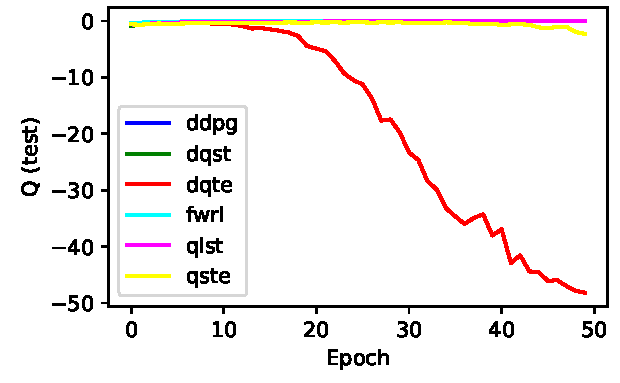
\includegraphics[width=\frac\columnwidth]{media/res/38f4625-FetchReach-v1-fwrl-future/test/mean_Q.pdf}%
  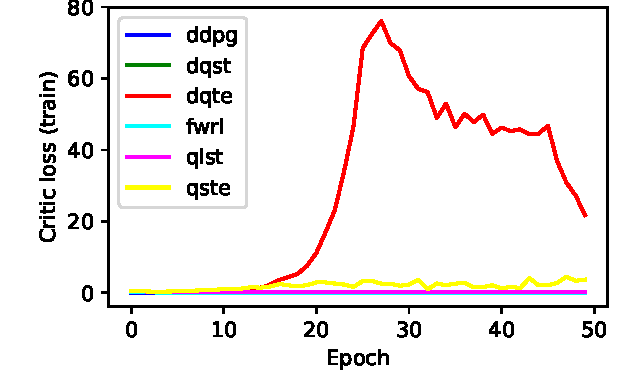
\includegraphics[width=\frac\columnwidth]{media/res/38f4625-FetchReach-v1-fwrl-future/train/critic_loss.pdf}\\
  On Fetch Slide\\
  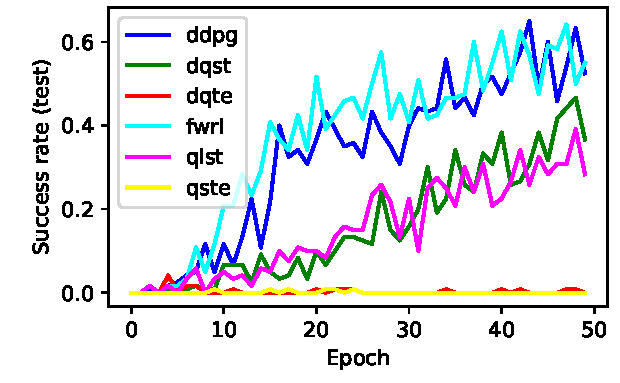
\includegraphics[width=\frac\columnwidth]{media/res/38f4625-FetchSlide-v1-fwrl-future/test/success_rate.pdf}%
  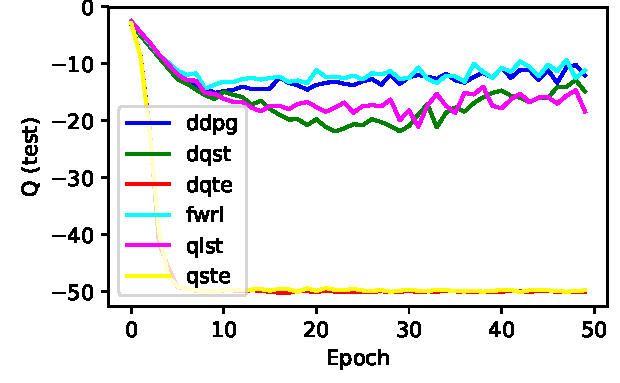
\includegraphics[width=\frac\columnwidth]{media/res/38f4625-FetchSlide-v1-fwrl-future/test/mean_Q.pdf}%
  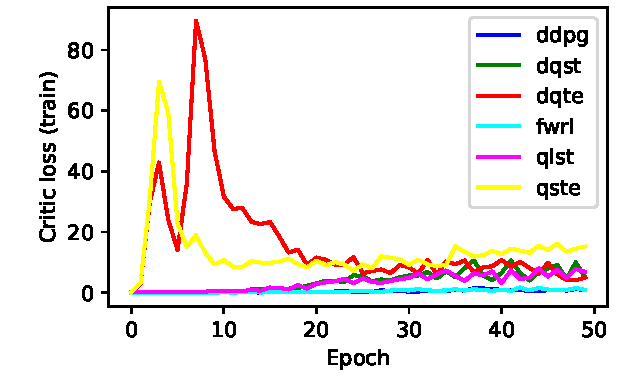
\includegraphics[width=\frac\columnwidth]{media/res/38f4625-FetchSlide-v1-fwrl-future/train/critic_loss.pdf}%
  On Fetch Pick and Place\\
  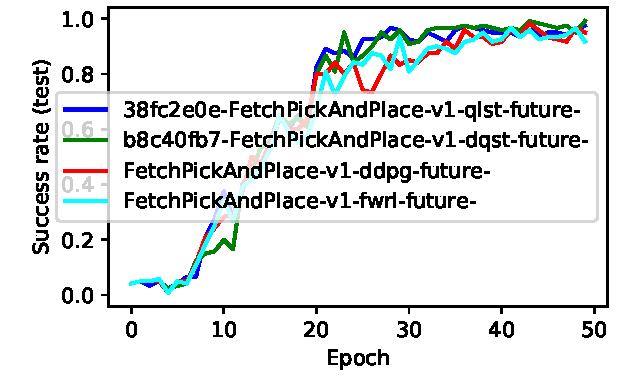
\includegraphics[width=\frac\columnwidth]{media/res/38f4625-FetchPickAndPlace-v1-fwrl-future/test/success_rate.pdf}%
  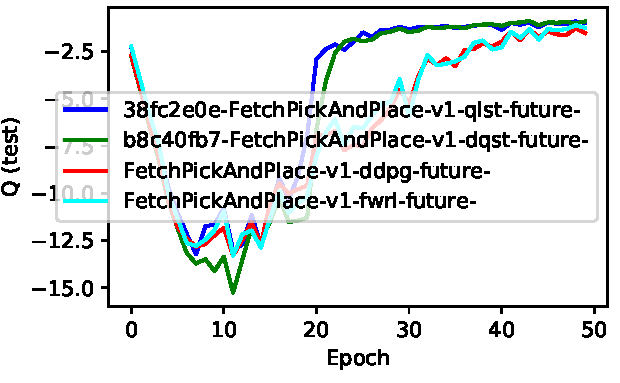
\includegraphics[width=\frac\columnwidth]{media/res/38f4625-FetchPickAndPlace-v1-fwrl-future/test/mean_Q.pdf}%
  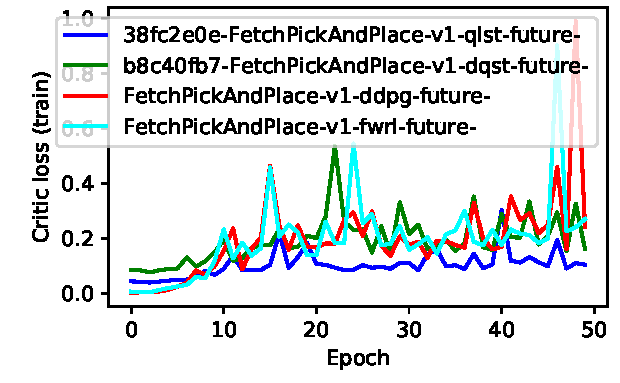
\includegraphics[width=\frac\columnwidth]{media/res/38f4625-FetchPickAndPlace-v1-fwrl-future/train/critic_loss.pdf}%
  On HandReach\\
  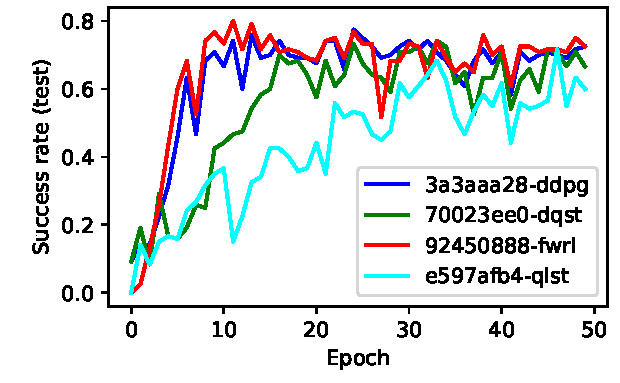
\includegraphics[width=\frac\columnwidth]{media/res/38f4625-92450888-HandReach-v0-fwrl-future/test/success_rate.pdf}%
  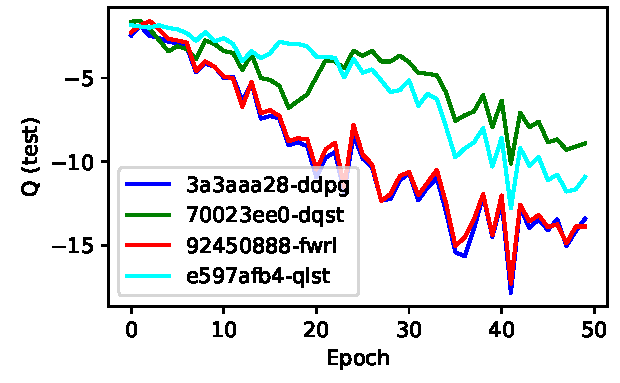
\includegraphics[width=\frac\columnwidth]{media/res/38f4625-92450888-HandReach-v0-fwrl-future/test/mean_Q.pdf}%
  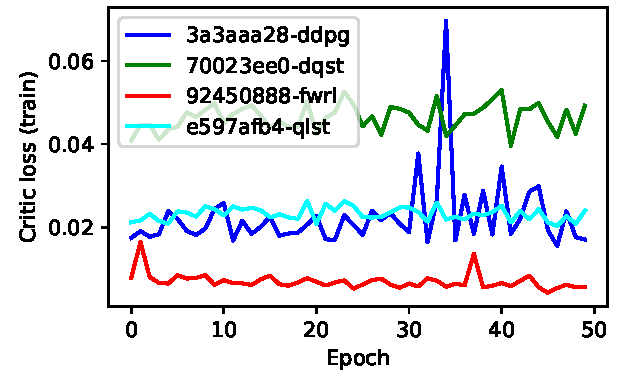
\includegraphics[width=\frac\columnwidth]{media/res/38f4625-92450888-HandReach-v0-fwrl-future/train/critic_loss.pdf}%
  \caption{
    Fetch results. Loss function changes do no seem to make a difference.
    There are four parts to the loss function (1) DDPG Loss $\LossDDPG$ ,
    (2) Step loss$\LossStep$,  
    (3) Lower bound $\LossLo$ and
    (4) Upper bound $\LossUp$ .
    ddpg = $\LossDDPG$,
    dqst = $\LossDDPG$ + $\LossStep$,
    fwrl = $\LossDDPG$ + $\LossLo$ +
    $\LossUp$,
    qlst = $\LossDDPG$ + $\LossStep$ + $\LossLo$ + $\LossUp$,
    dqte = $\LossDDPG$ + $\LossTrieq$,
    qste = $\LossDDPG$ + $\LossStep$ + $\LossTrieq$.
    Success rate is the fraction of times the agent reaches the goal. Q(test) is
    the estimated cumulative reward by the network. Critic loss is the total
    loss plotted during training.
    Because stfw, stlo, stup fail to succeed, we infer that the $\LossDDPG$ DDPG loss is
    critical for making the algorithm work. Since the qlst works better than
    fwrl, we infer that $\LossStep$ Step loss is also important.
    only.
    Since there is slight improvement in dqst over ddpg, this means
    $\LossStep$ really helps. dqst did not run fully but it shows
    promise (I need to fix a bug).
    But why does the loss for stfw keep rising? Does it mean that the SGD is not
    able to optimize the loss gradients in the right direction?
  }%
  \label{fig:fwrl-stepfwrl-noop-FetchPush}%
\end{figure}%
% 

%
\begin{figure}%
  \def\frac{0.25}
  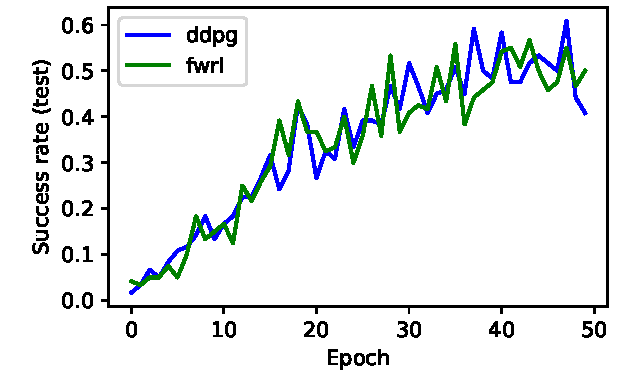
\includegraphics[width=\frac\columnwidth]{media/res/3d07a6e-FetchReachPR-v1-fwrl-future/test/success_rate.pdf}%
  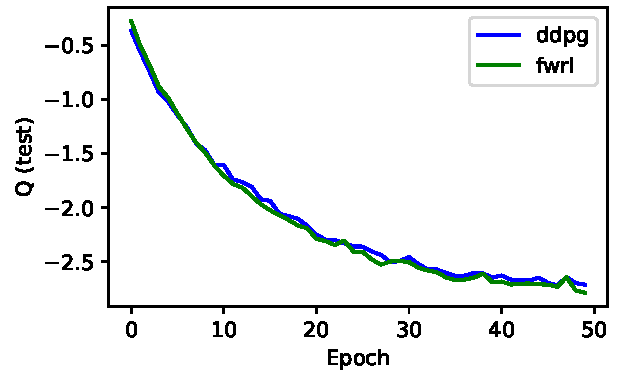
\includegraphics[width=\frac\columnwidth]{media/res/3d07a6e-FetchReachPR-v1-fwrl-future/test/mean_Q.pdf}%
  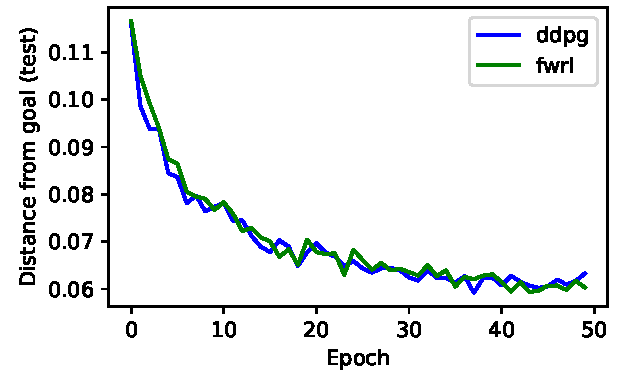
\includegraphics[width=\frac\columnwidth]{media/res/3d07a6e-FetchReachPR-v1-fwrl-future/test/ag_g_dist.pdf}%
  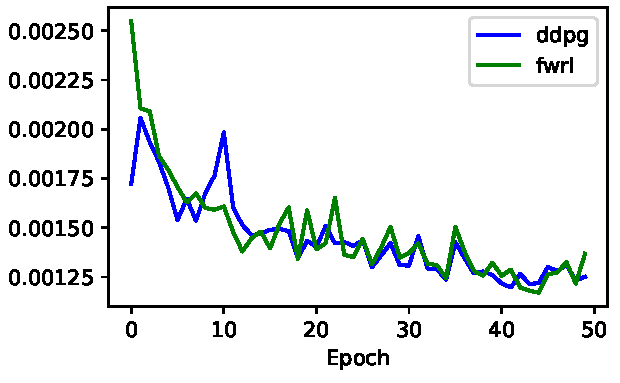
\includegraphics[width=\frac\columnwidth]{media/res/3d07a6e-FetchReachPR-v1-fwrl-future/train/critic_loss.pdf}%
  \label{fig:path-rewards}%
  \caption{Experiment to see the effect of only path rewards on loss terms. We
    did not include a step term which becomes very important in this case.}%
\end{figure}%
% 

%
\begin{figure}%
  \def\frac{0.24}
  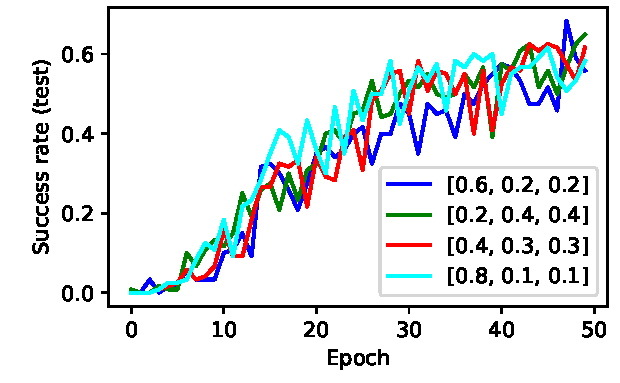
\includegraphics[width=\frac\columnwidth]{./media/res/04a8fc6-814a3d24-FetchSlide-v1-fwrl-future/test/success_rate.pdf}%
  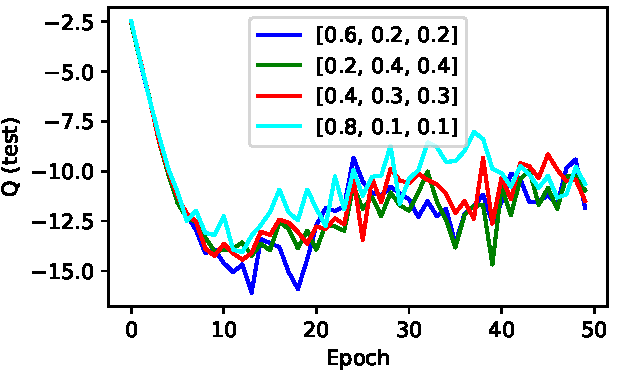
\includegraphics[width=\frac\columnwidth]{./media/res/04a8fc6-814a3d24-FetchSlide-v1-fwrl-future/test/mean_Q.pdf}%
  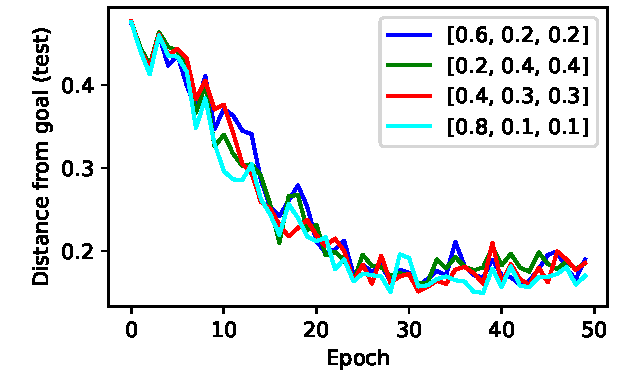
\includegraphics[width=\frac\columnwidth]{./media/res/04a8fc6-814a3d24-FetchSlide-v1-fwrl-future/test/ag_g_dist.pdf}%
  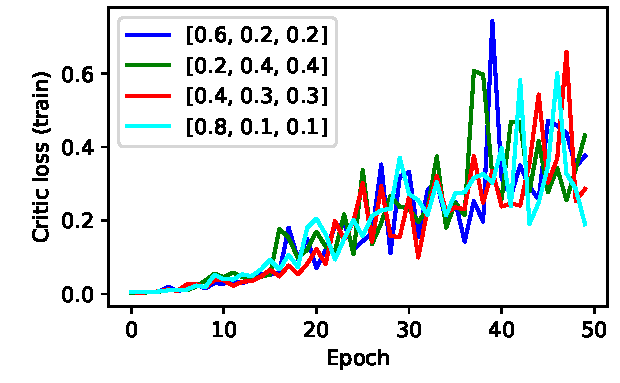
\includegraphics[width=\frac\columnwidth]{./media/res/04a8fc6-814a3d24-FetchSlide-v1-fwrl-future/train/critic_loss.pdf}%
  \label{fig:loss-term-weights}%
  \caption{Effect of weighted combination of loss terms on FetchSlide. The three
  loss terms being weighed in order are $[\LossDDPG, \LossLo, \LossUp]$}%
\end{figure}%
% 
We compared weighted combination of loss terms


%\subsection{Unanswered questions and things to try}
%
%\subsubsection{FWRL specific sampling}
%Right now the shuffle step in the algorithm is totally random and probably
%introduces more noise in the algorithm than it helps. A modification of HER
%sampling would sampling three time steps from the trajectory (single episode)
%$t_1 > t_2 > t_3$ and use $t_2$ as the intermediate state for
%$\LossUp$ and $\LossLo$.
%
%
%\subsubsection{Why is any loss term with upper/lower worse?}
%This is probably answered by  the above section but what are the other
%explanations. The total ``Critic loss'' is increasing for stfw
%($=\LossStep$ + $\LossLo$ + $\LossUp$),
%which seems to say that with $\LossDDPG$, it is hard to optimize the functions.
%
%
%\subsection{Is it still a contribution if the upper and lower bounds do not
%  improve the results?}
%Can we claim that this alternative formulation is new and more principled than HER?
